\section{SwitchCrypt Design} \label{sec:design}

What follows is a brief overview of SwitchCrypt's design
(\cref{subsec:overview}). We then discuss our novel, general API for
\emph{decoupling} the cipher implementations from the encryption/decryption
process (\cref{subsec:api}), describe and contrast three cipher \emph{switching
strategies} (\cref{subsec:strategies}), and then detail our scheme to
\emph{quantify} cipher strength (\cref{subsec:quantify}). Finally, we revisit
the battery saver example and summarize how the SwitchCrypt components fit
together (\cref{subsec:summary}). In this section, we first give a brief
overview of SwitchCrypt's design.

\subsection{SwitchCrypt Overview} \label{subsec:overview}

Like StrongBox, SwitchCrypt sits between a Log-structured File System (LFS) and
the backing storage, dividing it into a series independent same-size logical
units called \emph{nuggets}. A nugget consists of one or more contiguous
physical drive blocks with per-nugget metadata indicating which cipher was used
to encrypt the nugget.

SwitchCrypt uses the nugget layout to 1) track, detect, and handle overwrites,
2) limit the maximum length of any plaintext input to ciphers, thus amortizing
the overhead incurred during encryption~\cite{StrongBox}, and 3) independently
switch the cipher used to crypt individual nuggets.

\PUNT{\begin{figure}[t]
\centering
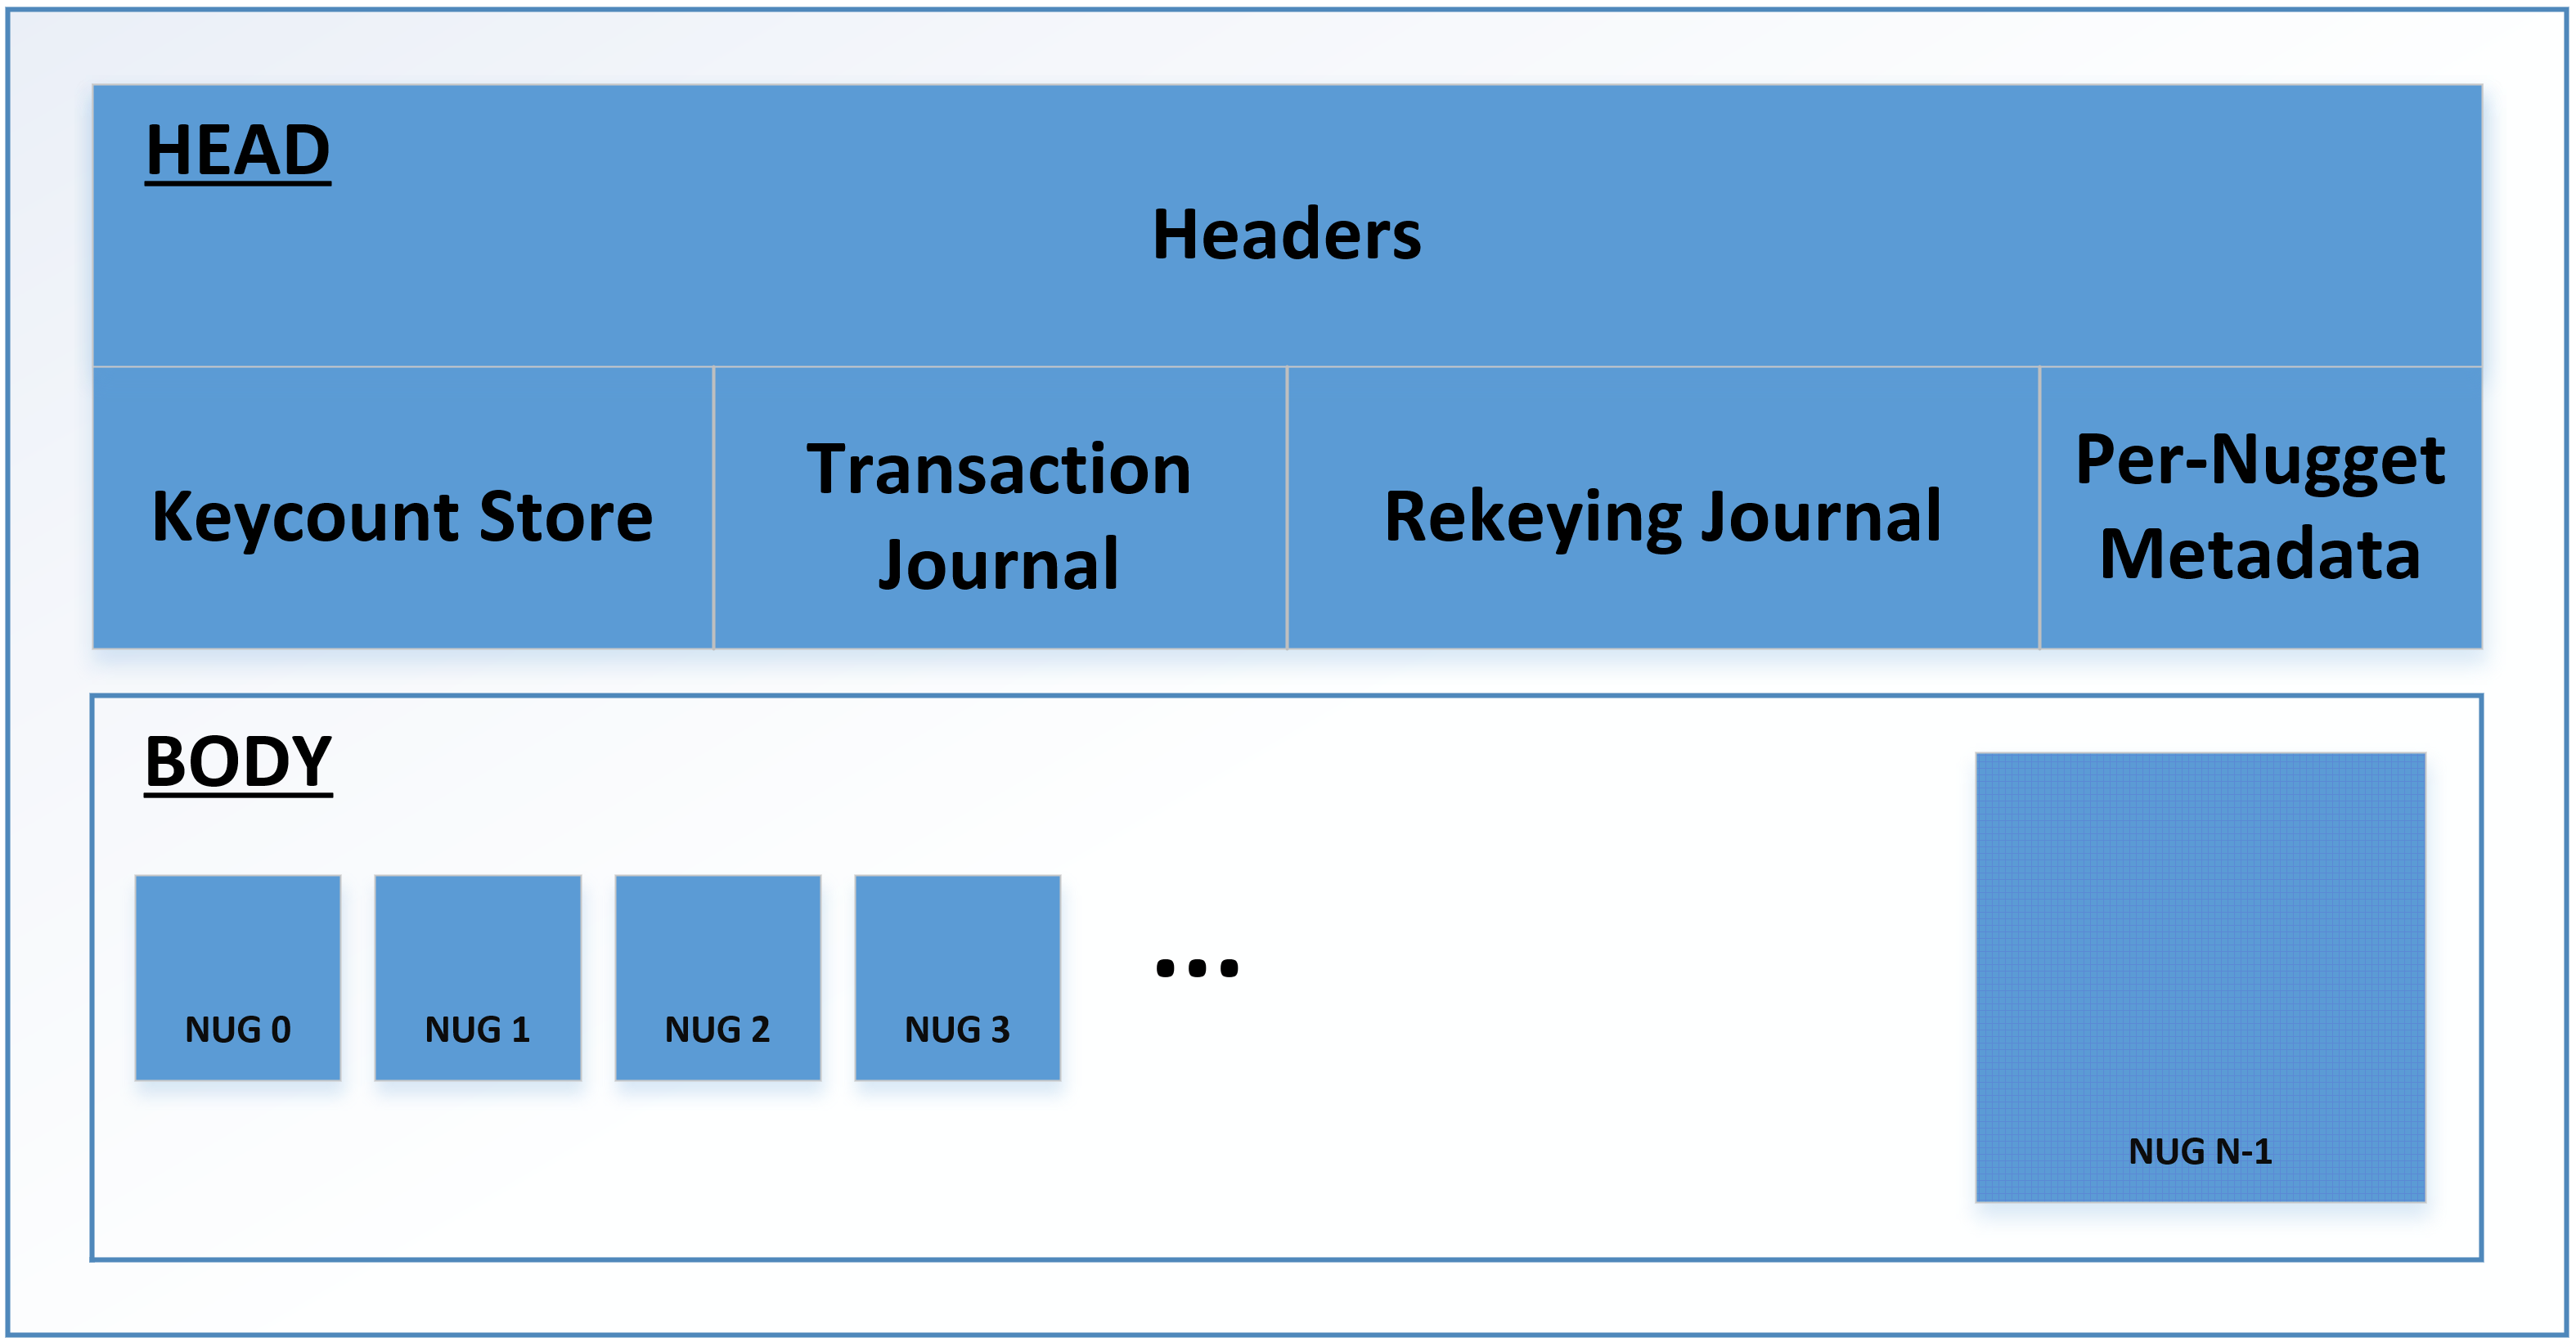
\includegraphics[width=\linewidth]{backstore.png}
 \caption{Layout of SwitchCrypt's backing storage.}\label{fig:backstore2}
\end{figure}}

\begin{figure}[ht]
   \centering
   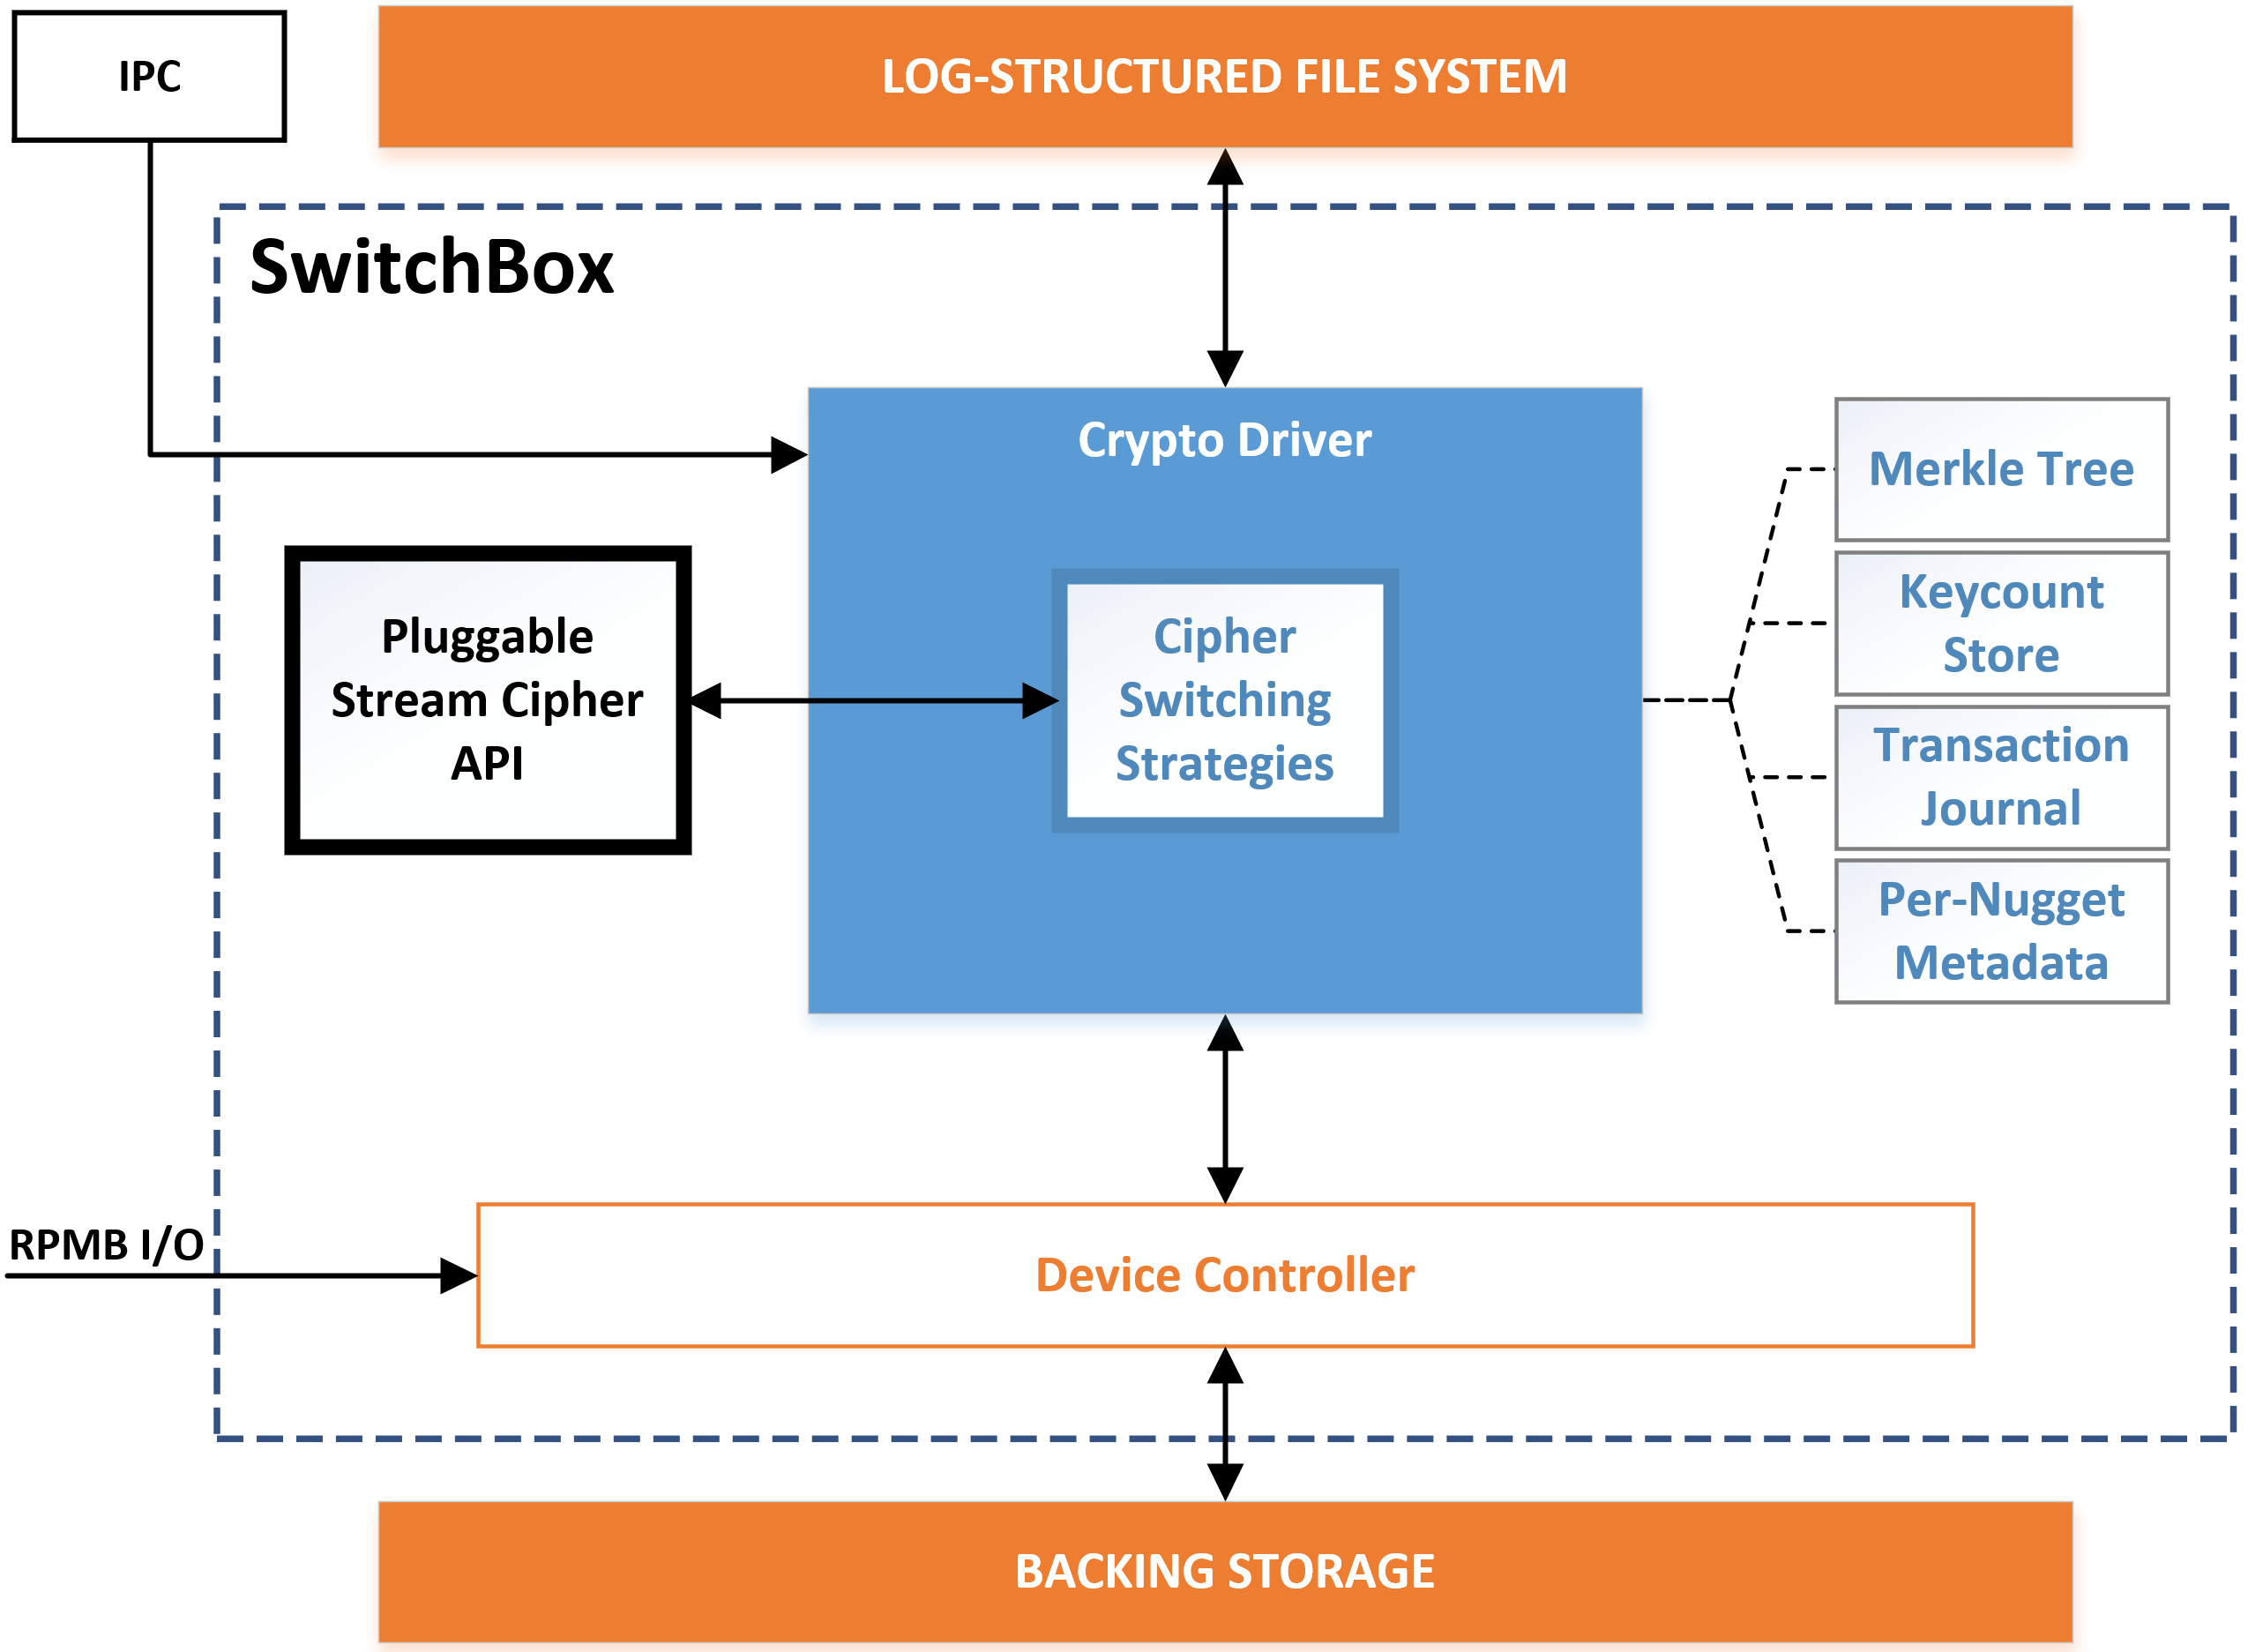
\includegraphics[width=\linewidth]{overview.png}
   \caption{Overview of the SwitchCrypt construction.}\label{fig:overview}
\end{figure}

\figref{overview} provides an overview of the SwitchCrypt design. SwitchCrypt is
composed of the cryptographic driver---responsible for executing our
\emph{switching strategies}---and six components. The first four components
belong to StrongBox: an in-memory \emph{merkle tree}; two drive-backed byte
arrays, \ie{the \emph{keycount store} and the \emph{transaction journal}}; a
globally persistent cryptographically secure monotonic counter~\cite{StrongBox}.
Our design adds the final two components: a flexible drive-backed store for
cipher-specific \emph{per-nugget metadata} and the \emph{generic stream cipher
API}.

The \emph{merkle tree} ensures the integrity of all data on a per-nugget level.
The \emph{keycount store} keeps track of each nugget's 64-bit cryptographic key.
The \emph{transaction journal} keeps track of writes to nuggets, allowing
SwitchCrypt to detect and respond to overwrites. The \emph{monotonic counter} 
prevents the system state from being rolled back. The \emph{per-nugget
metadata} is a drive-backed array where extra cryptographic material is stored
depending on the cipher used to encrypt the nugget. The size of the array is
determined by ciphers loaded through the \emph{generic stream cipher API}.

\subsection{Generic Stream Cipher API} \label{subsec:api}

There are \emph{many} ciphers we might use with SwitchCrypt, each with various
input requirements and output considerations. A key difference with prior work 
is that SwitchCrypt
must be able to encrypt and decrypt arbitrary nuggets without worrying about a
cipher's implementation details; prior approaches could have cipher-specific 
implementations because they did not consider switching.   
Thus, the cipher-specific details
must be handled with care or security is violated. With our
novel cipher API, we present an interface that \emph{decouples} cipher
implementations from the encryption/decryption process. This allows any cipher
to be integrated into SwitchCrypt without modification or special
considerations. Hence, different stream ciphers become interchangeable when they
would normally be incompatible, preventing us from trading them off one another.

The API is accessible at three levels:

\begin{enumerate}
   \item \textbf{\texttt{crypt\_data}}\\\texttt{crypt\_data}
   operates at a fine-grain level independent of SwitchCrypt's internals.
   Implementations receive an index and offset and are expected to return some
   number of bytes, \ie{a keystream}, which is XORed with nugget contents. At
   this level, there is no distinction made between encryption and decryption
   since both are accomplished with a simple XOR. This API level has the lowest
   implementation overhead and least flexibility.

   \item \textbf{\texttt{crypt\_data\_low}}\\\texttt{crypt\_data\_low}
   is identical to \texttt{crypt\_data} but provides a slightly lower level of
   abstraction when accessing the backing store, giving implementations more
   control over the XORing process. This is useful for less flexible ciphers but
   comes at the cost of increased implementation overhead.

   \item \textbf{\texttt{read\_data}} and \textbf{\texttt{write\_data}}\\
   These operate at a coarse-grain level tightly integrated with SwitchCrypt
   internals. Implementations are expected to handle all stages of cipher
   switching manually. Unlike the other two levels, encryption and decryption
   are distinct concerns. \texttt{read\_data} handles decryption during reads.
   \texttt{write\_data} handles encryption during writes. In exchange for
   maximum flexibility, there is significant implementation overhead with this
   approach.
\end{enumerate}

Were we using simple ciphers exclusively, \ie{those that do not differentiate between
encryption and decryption and always produce output of the same length as the
input}, we could generate a keystream and XOR it with data without the
the need for a new a API. However, some cipher implementations treat
encryption and decryption as two distinct operations. Others require different
parameters or special considerations before XORing the keystream with data.
Others produce extra output that must be stored during encryption and fetched
during decryption. Others exhibit some combination of these concerns. Our API
presents the cryptographic driver with a single unified interface where these
disparate concerns are abstracted away, laying the groundwork for
\emph{cipher switching}.

\subsection{Cipher Switching Strategies} \label{subsec:strategies}

The SwitchCrypt design allows many differently-ciphered storage units to
co-exist on the backing store. However, at any moment, there is a single
\emph{active cipher} configuration. The active cipher is the only cipher used to
encrypt nugget contents. When a cipher switch occurs, a different cipher becomes
the active cipher. At this point, SwitchCrypt must determine \emph{when} to
re-cipher a nugget and \emph{where} to store the output on the drive.
``Re-ciphering'' here means using a non-active cipher to decrypt a nugget's
contents and using the active cipher to re-encrypt them. Depending on
 the use case, it may make the most sense to re-cipher a nugget
immediately, or eventually, or to maintain several areas of differently-ciphered
nuggets concurrently.

A naive approach would immediately switch every nugget to the desired cipher,
but the latency and energy cost would be unacceptable. Hence, a more adaptable
approach is necessary: cipher \emph{switching strategies}. These strategies
allow re-ciphering nuggets in a variety of cases with minimal impact on
performance and battery life, without compromising data security.

Determining \emph{when} to target a nugget for re-ciphering we call
\emph{temporal switching}, for which we propose the \emph{Forward} switching
strategy. Determining \emph{where}---in which storage region and across which
nuggets--to output ciphertext we call \emph{spatial switching}, for which we
propose the \emph{Mirrored} and \emph{Selective} switching strategies.

\textbf{A) Forward Switching Strategy.} When a nugget is encountered during I/O
that is encrypted using a cipher other than the active cipher, the Forward
strategy dictates that this nugget be re-ciphered immediately. If a particular
nugget encrypted with a non-active cipher configuration is never encountered
during I/O, it is never re-ciphered and remains on the backing store in its
original state. In this way, the Forward strategy represents a form of temporal
cipher switching.

Rather than re-cipher the entire backing store every time the active cipher
configuration changes, this strategy limits the performance impact of cipher
switching to individual nuggets. The expense of re-ciphering is paid only once,
after which the nugget is accessed normally during I/O until the active cipher
configuration is switched again.

\PUNT{There are several forms the Forward strategy might take. The default and
most intuitive is \emph{0-forward}, in which SwitchCrypt immediately transitions
individual nuggets encountered during I/O to the active cipher configuration if
they are not using it. Over time, if various I/O operations end up touching
every nugget in the backing store, the encrypted contents of every nugget will
become decryptable with the currently active cipher configuration.

The Forward strategy might also take the form of \emph{N-forward}, where
SwitchCrypt attempts to take advantage of spatial sequential locality to
transition whole sets of nuggets into the active cipher configuration. We can
trivially expand the forward strategy to encompass the entire backing store by
selecting $N$ equal to the total number of nuggets managed by SwitchCrypt. This
would have the overhead of re-ciphering large swaths of the backing store upon
every I/O operation where a nugget encrypted with the non-active cipher
configuration is encountered. Of course, this has the same dire implications for
performance as simply re-initializing the entire system or encrypted
container with the new cipher.}

\textbf{B) Selective Switching Strategy.} When SwitchCrypt is initialized with
the Selective strategy, the backing store is partitioned into $C$ regions where
$C$ represents the maximum number of ciphers; each regions' nuggets are
encrypted by each of the $C$ ciphers respectively. For instance, were
SwitchCrypt initialized using two ciphers ($C = 2$), the backing store would be
partitioned in half; all nuggets in the first region would be encrypted with the
first cipher while all nuggets in the second would be encrypted with the other.

Hence, unlike the Forward strategy, which schedules individual nuggets to be
re-ciphered at some point in time after the active cipher configuration is
switched, the Selective strategy allows the wider system to indicate
\emph{where} on the backing store a read or write operation should occur. In
this way, the selective strategy represents a form of spatial cipher switching
where different regions of the backing store can store differently-ciphered
nuggets. A user could take advantage of this to, for instance, set up regions
with different security properties and performance characteristics, managing
them as distinct virtual drives or even reading/writing bytes to different
security regions on the same drive.

Regions of the backing store will not be in a consistent state and will likely
contain different data.

\textbf{C) Mirrored Switching Strategy.} Similar to the Selective strategy, when
SwitchCrypt is initialized with the Mirrored strategy, the backing store is
partitioned into $C$ regions where $C$ represents the maximum number of ciphers;
each regions' nuggets are encrypted by each of the $C$ ciphers respectively.

However, unlike the Selective strategy, all write operations that hit one
region are mirrored into the other regions immediately. The mirrored
strategy allows the wider system to indicate (via the active cipher) within
which region a \emph{read} operation should occur. In this way, the Mirrored
strategy represents a form of spatial cipher switching. A user could take
advantage of this to \emph{quickly} converge the backing store to a single
cipher configuration without loss any data or the performance penalty of
re-ciphering an entire region's nuggets.

All regions of the backing store will always be in a consistent state and always
share the same data.

\subsubsection{Comparing Cipher Switching Strategies}

\begin{table}[]
   \begin{tabular}{@{}|c|c|c|C{25mm}|@{}}
      \toprule
      \textbf{Strategy} & \textbf{Convergence} & \textbf{Waste} & \textbf{Performance} \\ \midrule
      Forward   & Slow           & Low  & Fast reads and writes unless switching \\
      \hline
      Mirrored  & Nearly instant & High & Fast reads; slow writes \\
      \hline
      Selective & Slow           & High & Fast reads and writes  \\
      \hline
   \end{tabular}
   \caption{A summary comparison between the three cipher switching strategies.}
   \label{tbl:strategies-advantages}
\end{table}

\tblref{strategies-advantages} summarizes the tradeoffs between the three cipher
switching strategies.

\textbf{Convergence.} Depending on the use case, the ability to quickly converge
the entire backing store to a single cipher configuration without losing data is
very useful (see: \secref{usecases}). The near-instantaneous nature of SSD
Instant Secure Erase (ISE) implementations on modern SSDs~\cite{ISE1,ISE2,ISE3}
makes this a very fast process for the Mirrored strategy. The Forward strategy
is slow to converge compared to Mirrored since, in the worse case, every nugget
on the drive will require re-ciphering. The Selective strategy is similarly slow
to converge since entire regions of nuggets must be re-ciphered to prevent data
loss; those regions can be destroyed with ISE too, which would be very fast, but
unlike Mirrored the data would be lost forever, which is rarely desirable.

\textbf{``Waste''.} Unlike the other two strategies, using the Forward strategy
does not dramatically reduce the total usable space on the drive by the
end-user. This is because the Forward strategy allows differently-ciphered
nuggets to co-exist contiguously on the backing store. Since the Mirrored and
Selective strategies require partitioning the backing store into some number of
regions---where the writeable size reported back to the OS is some function of
region size---there is a necessary reduction in usable space.

\textbf{Performance.} The Selective and Mirrored strategies can read data from
the backing store with low overhead, reaching performance parity with prior
work. This is because switching ciphers using these strategies amounts to
offsetting the read index so it lands in the proper region, which has little
overhead. The Forward strategy also reads with low overhead except in the case
where a nugget was not encrypted with the active cipher. This triggers
re-ciphering, which can be costly if the workload touches unique nuggets and is
small enough that cost is not amortized.

The Selective strategy also writes with low overhead because, like with reads,
an offset is the only requirement. The Mirrored strategy, on the other hand, can
be two or more times slower for writes (when $C = 2$) compared to baseline. Each
additional region ($C > 2$) compounds the write penalty. This is because each
writes is ``mirrored'' across all regions. As with reads, the Forward strategy
writes with low overhead except in the case where a nugget was not
encrypted with the active cipher configuration. This triggers costly
re-ciphering, which can compound depending on workload.\\

With these tradeoffs in mind: Mirrored is ideal when the backing store must
converge quickly, write performance is not the primary concern, and drive space
is abundant; Selective is ideal when different data should be encrypted
differently and drive space is abundant; and Forward is ideal when some subset
of nuggets should be encrypted differently without wasting drive space. See
\secref{usecases} for specific scenarios that highlight the practical difference
between strategies.

\subsubsection{Threat Model for Cipher Switching Strategies}

The primary concern facing any FDE solution is that of confidentiality: an
adversary should not be able to decrypt encrypted plaintext without the right
key. With this research, we select five cipher implementations and configure
them under SwitchCrypt: ChaCha~\cite{ChaCha20} (ChaCha8 and ChaCha20), and
Freestyle~\cite{Freestyle} in fast, balanced, and secure configurations (see:
\secref{implementation}). Each cipher has been proven formally secure in that
there are no known efficient attacks against them.

Encryption is achieved via a binary additive approach: cipher output (keystream)
is combined with plaintext nugget contents using XOR, with metadata to track
writes and ensure that pad reuse never occurs during overwrites and that the
system can recover from crashes into a secure state~\cite{StrongBox}.

Another concern is data integrity: an adversary should not be able to tamper
with ciphertext and it go unnoticed. As with prior work, we use an in-memory
Merkle Tree to ensure nugget and system integrity~\cite{StrongBox}.

Switching strategies add an additional concern: even if we initiate a ``cipher
switch,'' there may still be data on the backing store that is encrypted with a
non-active cipher configuration. Is this a problem? For the Forward strategy,
this implies data may at any time be encrypted using the least desirable cipher.
For the Mirrored and Selective strategies, the backing store is partitioned into
regions where nuggets are guaranteed to be encrypted with each cipher. However,
in terms of confidentiality, all the ciphers we configured under SwitchCrypt
have been proven formally secure. Hence, nuggets encrypted with different secure
ciphers can co-exist on the backing store securely, depending on the use case
(see: \secref{usecases}).

\subsection{Quantifying Cipher Security Properties} \label{subsec:quantify}

Every cipher mentioned in this paper is considered secure in that \emph{there
are no known practical attacks against them}~\cite{All, Ciphers, Again}. This
implies data is kept confidential versus any adversary, however it is often
desirable to secure data at rest in special contexts or considering future
adversaries with abundant resources. In this way, a cipher that is more
resilient to cryptanalysis or brute-force or round count than is currently
required or a cipher that elegantly handles nonce-reuse might be more desirable.

To simplify reasoning about trading off such disparate cryptographic properties
in the FDE context, we must have a way to quantitatively compare a cipher's
``desirability'' for SwitchCrypt and for FDE more broadly. Hence, we do not
attempt to define a generally applicable \textit{ranking} of \emph{security
strength}. Instead, we score ciphers (\ie{a so-called ``security score''}) based
on three key security properties that, when summed, give a relative estimate of
the difficulty (or resources required) to attack data secured under SwitchCrypt
FDE (see: \tblref{security-quant}).

Our scoring scheme is a combination of well understood schemes: scoring ciphers
on their confusion and diffusion of plaintext bits during
encryption~\cite{MicrosoftCryptanalysisAES,SchneiersOnRounds} (commonly known as
\emph{round count}), on how they behave when given the same input
parameters~\cite{random-output1,Freestyle,random-output2} (normally an
unacceptable confidentiality-breaking overwrite condition), and on there being
penalties for supplying the wrong key when attempting to decrypt (\ie{an
attacker should have to do more work than the
defender})~\cite{scrypt,Freestyle,others2}.

\textbf{1) Output randomization (OR).} A cipher with output randomization
generates different ciphertexts non-\\deterministically given the same key,
nonce, and message. This makes chosen-ciphertext (CCA) and other attacks where
the ciphertext is in full control of the adversary much more
difficult~\cite{Freestyle}.

This is a binary feature in that a cipher either outputs deterministically given
the same input or it does not. A cipher with non-deterministic output given the
same key, nonce, and message as inputs scores a 1 for this feature while a
cipher with deterministic output given the same input scores a 0.

\textbf{2) Resistance to brute force and offline/dictionary attacks (RBF).} We
narrowly define ``standard resistance'' versus brute-force and
offline/dictionary attacks with respect to the time taken to finish decrypting
ciphertext given an incorrect key versus a correct key; a cipher with standard
resistance to brute force and offline/dictionary attacks has no kind of
\emph{key-guessing penalty}~\cite{Freestyle}---the ciphertext is decrypted no
slower when given the incorrect key versus the correct key. Similarly, we
consider ciphers with so-called ``enhanced resistance,'' where they are expected
to take longer to finish decrypting ciphertext given an incorrect key versus a
correct key with high probability. This property is also useful in instances
where SwitchCrypt is initialized with a weak password/key.

Scores for this feature range from 0 to 1, where 0 represents no resistance, 0.5
is standard resistance to brute-force and offline/dictionary attacks, and 1 is
the aforementioned ``enhanced resistance''.

\textbf{3) Relative round count and key length (RR/RK).} The ciphers we examine
in this research are all constructed around the notion of \emph{rounds}, where a
higher number of rounds or longer key typically imply a stronger confidentiality
guarantee given there are no fatal related-key attacks. This feature represents
how many rounds the cipher executes compared to the accepted ``standard'' round
count for that cipher. For instance: ChaCha8 is a reduced round version of the
standard ChaCha20, both using 256-bit keys.

Scores for variants are distributed evenly from 0-1. For instance, ChaCha8
scores 0 and ChaCha20 scores 1\@.

\begin{table}[]
  \begin{tabular}{@{}lllll@{}}
  \toprule
  \textbf{Cipher} & \textbf{OR} & \textbf{RBF} & \textbf{RR/RK} & \textbf{score} \\ \midrule
  ChaCha8         & 0           & 0.5          & 0              & 0.5            \\
  %ChaCha12        & 0           & 0.5          & 0.5            & 1              \\
  ChaCha20        & 0           & 0.5          & 1              & 1.5            \\
  %Salsa8          & 0           & 0.5          & 0              & 0.5            \\
  %Salsa12         & 0           & 0.5          & 0.5            & 1              \\
  %Salsa20         & 0           & 0.5          & 1              & 1.5            \\
  %AES128-CTR      & 0           & 0.5          & 0              & 0.5            \\
  %AES256-CTR      & 0           & 0.5          & 1              & 1.5            \\
  %HC128           & 0           & 0.5          & 0              & 0.5            \\
  %HC256           & 0           & 0.5          & 1              & 1.5            \\
  Freestyle (F)   & 1           & 1            & 0              & 2              \\
  Freestyle (B)   & 1           & 1            & 0.5            & 2.5            \\
  Freestyle (S)   & 1           & 1            & 1              & 3
  \end{tabular}
  \caption{These ``scores'' represent a cipher's desirability to SwitchCrypt and
  to FDE more generally. Ciphers with OR can operate below overwrite
  protections, increasing performance; ciphers with RBF and high RR/RK have
  extra resilience against confidentiality attacks.}
  \label{tbl:security-quant}
\end{table}

\subsection{Putting It All Together} \label{subsec:summary}

We revisit the motivating example from \secref{motivation}. Initially, I/O
requests come down from the LFS and are received by the cryptographic driver,
which divides the request by which nuggets it touches. For each nugget, the
per-nugget metadata is consulted to determine with which cipher the nugget is
encrypted. If it is encrypted with the active cipher, which must be true if we
have not initiated a cipher switch, the write is handled similarly to prior
work: encrypted data is read in from backing storage, the merkle tree and
monotonic counter are consulted to ensure the integrity of encrypted data, the
transaction journal is consulted during write operations so that overwrites are
handled and pad reuse violations are avoided, and then the keycount store is
consulted to derive the nugget's unique encryption key from some master secret.
Using the generic stream cipher API to call out to the active stream cipher
implementation, SwitchCrypt encrypts/decrypts the nugget's contents and commits
any updates back to storage~\cite{StrongBox}.

When the device enters ``battery saver'' mode, the energy monitoring software
downclocks the CPU and indicates to SwitchCrypt that a more energy-efficient
cipher should be used until we return to a non-curtailed energy budget. Now,
when the cryptographic driver divides I/O requests into each affected nugget,
the per-nugget metadata shows SwitchCrypt that the nugget is encrypted using a
cipher that is not the active cipher. This triggers the re-ciphering code path.
Since we are using the Forward switching strategy, this means the nugget data is
immediately decrypted by calling out to the inactive cipher through the API and
then re-encrypted by calling out to the active cipher. Depending on the API
level the cipher is implemented at, either 1) the cryptographic driver manages
encrypting/decrypting data and updating the merkle tree and monotonic counter,
transaction journal, and keycount store or 2) the cipher implementation handles
updating SwitchCrypt internals directly. Afterwards, the I/O operation is
committed to the backing store.
